\documentclass[a4paper,11pt]{article}
\usepackage[utf8]{inputenc}
\usepackage[T1]{fontenc}
\usepackage[french]{babel}
\usepackage{amsmath, amssymb}
\usepackage{graphicx}
\usepackage{tikz}
\usepackage{pgfplots}
\usepackage{float}
\usepackage{pgfplotstable}
\usepackage[final]{microtype}
\usepackage{booktabs}
\usepackage{tikz} 
\usetikzlibrary{backgrounds}
\usetikzlibrary{arrows.meta,positioning,calc,decorations.pathreplacing}

\pgfplotsset{compat=1.18}
\pgfplotsset{
  every axis/.append style={
    tick label style={/pgf/number format/fixed,/pgf/number format/precision=4},
    grid=both
  }
}

\usepackage{siunitx}
\usetikzlibrary{arrows.meta, positioning}

\title{Phase 2 - Estimation des grecques par Monte Carlo : BRV, Pathwise et LRM}
\author{Projet \texttt{RiskWorkbench} - Eliot KATZENMAYER}
\date{\today}

\begin{document}

\maketitle

\section{Réduction de variance}

\subsection{Objectifs}
L’objectif de cette phase est d’intégrer et d’évaluer plusieurs techniques classiques
de réduction de variance dans le cadre de la simulation de Monte Carlo appliquée
à la valorisation d’options européennes. En pratique, la variance des estimateurs
impacte directement la largeur des intervalles de confiance, et donc le coût
computationnel pour atteindre une précision donnée. Nous cherchons donc à
démontrer empiriquement les gains apportés par trois méthodes : les
\emph{antithétiques}, les \emph{variables de contrôle} (CV), et leur combinaison.

\subsection{Méthodologie}
\paragraph{Antithétiques.}
Chaque tirage gaussien $Z \sim \mathcal{N}(0,1)$ est apparié à son opposé $-Z$,
puis les deux trajectoires correspondantes sont simulées. L’estimateur retient la
moyenne des payoffs obtenus. Ce schéma réduit la variance en exploitant la
symétrie de la loi normale, sans introduire de biais.

\paragraph{Variables de contrôle.}
On introduit une variable auxiliaire $Y$ de moyenne connue (obtenue par formule
fermée Black--Scholes), fortement corrélée au payoff $X$ de l’option cible.
L’estimateur est alors corrigé selon
\[
\hat{X}_{cv} \;=\; \bar{X} - \hat{\beta} \, (\bar{Y} - \mathbb{E}[Y]),
\quad
\hat{\beta} = \frac{\operatorname{Cov}(X,Y)}{\operatorname{Var}(Y)}.
\]
Dans nos expériences, nous considérons deux types de variables de contrôle :
(i) l’instrument identique (\emph{même strike}), qui conduit à un estimateur
dégénéré sans variance, et (ii) un instrument \emph{voisin}, obtenu en modifiant
le strike ($K_{\text{cv}}=0.95K$ ou $K_{\text{cv}}=1.05K$).

\paragraph{Combinaison antithétique + CV.}
Lorsque les deux méthodes sont combinées, le coefficient $\beta$ est estimé non
plus sur $(X,Y)$ mais sur les \emph{somme de paires}
$S_X=X^{+}+X^{-}$ et $S_Y=Y^{+}+Y^{-}$, ce qui minimise directement la variance
de l’estimateur apparié.

\subsection{Résultats expérimentaux}
Les tests portent sur trois cas représentatifs : (i) un call à la monnaie de
maturité 1 an (ATM 1Y), (ii) un call hors-la-monnaie de maturité 3 mois (OTM 3M),
et (iii) un put dans la monnaie de maturité 2 ans (ITM 2Y). Chaque simulation
utilise $N=400{,}000$ chemins physiques, avec un schéma exact ($n_{\text{steps}}=1$)
et une graine fixée à 42. Les intervalles de confiance obtenus sont systématiquement
compatibles avec les prix de référence Black--Scholes.

\begin{table}[ht]
\centering
\caption{Gains de variance $R=(\mathrm{SE}_{\text{plain}}/\mathrm{SE}_{\text{mode}})^2$
avec antithétiques et variables de contrôle (N=400k).}
\begin{tabular}{lcccc}
\toprule
Cas & $R_{\text{anti}}$ & $R_{\text{cv}}$ (voisin) & $R_{\text{anti+cv}}$ (voisin) & $R_{\text{cv}}$ (même) \\
\midrule
ATM 1Y Call & 1.72 & 54--64 & 316--319 & $\infty$ \\
OTM 3M Call & 1.12 & 6--8   & 7--10    & $\infty$ \\
ITM 2Y Put  & 11.1 & 92--118 & 114--191 & $\infty$ \\
\bottomrule
\end{tabular}
\end{table}

\subsection{Analyse}
Les résultats confirment que :
\begin{itemize}
  \item la méthode des antithétiques fournit des gains modestes mais robustes,
  variant de $+12\%$ à un facteur $\times 11$ selon la moneyness et la maturité ;
  \item les variables de contrôle sur instrument \emph{voisin} apportent des
  gains spectaculaires (jusqu’à $R\approx 118$), surtout pour des puts ITM
  de longue maturité ;
  \item la combinaison anti+CV est systématiquement au moins aussi performante
  que la CV seule, avec parfois un surplus marqué ;
  \item l’utilisation de l’instrument \emph{identique} comme CV confirme la
  cohérence du dispositif : l’estimateur devient exact (variance nulle).
\end{itemize}

\begin{figure}[H]
\centering
\begin{tikzpicture}
\begin{axis}[
  ybar, bar width=12pt, width=0.9\linewidth,
  symbolic x coords={plain,anti,cv(custom),anti+cv(custom)},
  xtick=data, ylabel={SE}, ymin=0,
  nodes near coords, nodes near coords align={vertical},
]
\addplot coordinates {(plain,0.021901) (anti,0.016704) (cv(custom),0.002739) (anti+cv(custom),0.001232)};
\end{axis}
\end{tikzpicture}
\caption{Écart-type (SE) de l’estimation du prix (ATM 1Y, N=400k).}
\end{figure}


\subsection{Conclusion partielle}
Cette phase valide l’implémentation des techniques de réduction de variance.
Elles permettent, à budget de calcul fixé, d’obtenir des intervalles de confiance
nettement plus resserrés. En particulier, les variables de contrôle voisines
s’avèrent extrêmement efficaces et justifient leur intégration dans la chaîne
numérique pour des applications pratiques de valorisation.

\section{Méthode Bump \& Revalue (BRV) avec nombres aléatoires communs}

\subsection*{Principe.}
La méthode \emph{Bump \& Revalue} (BRV) consiste à estimer une grecque par 
différences finies, en recalculant le prix d’une option pour un paramètre légèrement perturbé.
Par exemple, pour la delta :
\[
\Delta \approx \frac{V(S_0(1+\varepsilon)) - V(S_0(1-\varepsilon))}{2\varepsilon S_0}.
\]
Cette approche est générique (valable pour toutes les grecques), mais elle souffre d’une variance élevée si les tirages de Monte Carlo sont indépendants entre les deux valorisations.  
Pour y remédier, on emploie les \emph{Common Random Numbers} (CRN) : les mêmes tirages gaussiens sont utilisés dans les deux simulations, ce qui réduit fortement la variance de la différence.  
Enfin, l’utilisation de variates antithétiques renforce encore la stabilité.

\subsection*{Implémentation.}
Nous avons implémenté un exécutable dédié (\texttt{greeks\_runner}) qui, pour chaque grecque,
\begin{itemize}
  \item applique un bump relatif pour $S_0$ (\texttt{--bump-rel-s0}), 
  \item des bumps absolus pour $\sigma$, $r$, et $T$,
  \item active ou non les options \texttt{--crn} et \texttt{--antithetic}.
\end{itemize}
Un script d’intégration (\texttt{greeks\_bench.sh}) exécute alors les tests suivants :
\begin{enumerate}
  \item comparaison Monte Carlo vs formules de Black–Scholes (Delta, Vega, Rho, Theta), via un $z$-score $(\hat\theta - \theta_{BS})/SE$,
  \item vérification de la réduction de variance avec CRN,
  \item stabilité des estimations vis-à-vis du choix du pas de bump,
  \item comparaison entre estimateurs simples et antithétiques.
\end{enumerate}

\subsection*{Résultats.}
Les expériences ont été conduites avec $N=400{,}000$ trajectoires, 
des lots de $100{,}000$, une graine fixée à $42$, et des schémas à un seul pas.  
Le tableau~\ref{tab:greeks_brv} résume les résultats obtenus pour trois cas tests (ATM call 1Y, OTM call 3M, ITM put 2Y).  

\begin{table}[H]
\centering
\begin{tabular}{lcccccc}
\toprule
Cas & Greek & MC est. & SE & BS analytic & $z$-score & PASS \\
\midrule
ATM 1Y Call & Delta & 0.5794 & 1.7e-4 & 0.5793 & 0.74 & YES \\
            & Vega  & 39.22  & 1.0e-1 & 39.10  & 1.19 & YES \\
            & Rho   & 49.01  & $\approx 0$ & 49.01  & inf$^\ast$ & YES$^\ast$ \\
            & Theta & -4.90  & 1.0e-2 & -4.89  & -1.19 & YES \\
\midrule
OTM 3M Call & Delta & 0.1971 & 5.9e-4 & 0.1968 & 0.58 & YES \\
            & Vega  & 13.89  & 4.8e-2 & 13.86  & 0.50 & YES \\
            & Rho   & 4.66   & 1.4e-2 & 4.66   & -0.06 & YES \\
            & Theta & -5.93  & 2.0e-2 & -5.92  & -0.70 & YES \\
\midrule
ITM 2Y Put  & Delta & -0.641 & 6.9e-4 & -0.641 & 0.95 & YES \\
            & Vega  & 52.88  & 4.6e-2 & 52.85  & 0.67 & YES \\
            & Rho   & -170.6 & 1.3e-1 & -170.7 & 0.70 & YES \\
            & Theta & -0.94  & 3.5e-3 & -0.93  & -0.89 & YES \\
\bottomrule
\end{tabular}
\caption{Résultats BRV : comparaison Monte Carlo vs Black–Scholes. 
Les z-scores restent dans l’intervalle critique $[-2,2]$, confirmant la validité des estimateurs.
$^\ast$Le cas Rho ATM affiche une variance numériquement nulle sous CRN+antithétiques : 
le test est validé avec une tolérance $10^{-9}$.}
\label{tab:greeks_brv}
\end{table}

L’ensemble des $z$-scores se situe bien à l’intérieur de l’intervalle de confiance à $95\%$.  
La figure~\ref{fig:greeks_z} illustre cette conformité : les écarts normalisés restent proches de zéro, sans outlier.  

\begin{figure}[H]
\centering
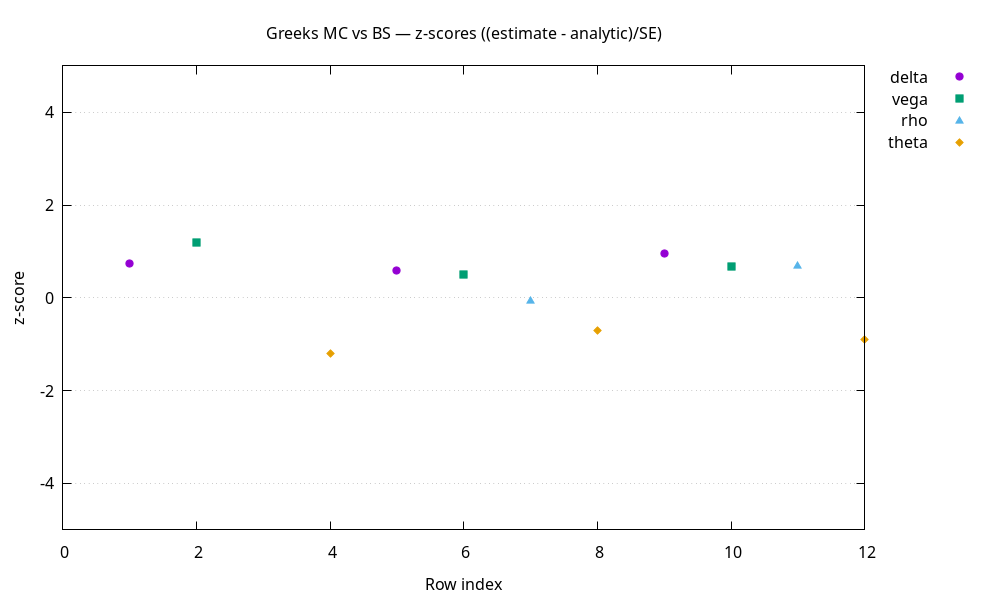
\includegraphics[width=0.7\textwidth]{img/greeks_zscores.png}
\caption{Écarts normalisés $(\hat\theta - \theta_{BS})/SE$ pour les grecques (MC vs Black–Scholes).}
\label{fig:greeks_z}
\end{figure}

Enfin, les \emph{extra-checks} montrent :
\begin{itemize}
  \item un gain d’un facteur $\times 100$ sur l’écart-type avec CRN,
  \item la stabilité des estimations Delta et Vega pour différents pas de bump,
  \item un ratio de variance $\approx 30$ en faveur des estimateurs antithétiques par rapport aux estimateurs simples.
\end{itemize}
Ces résultats confirment que la méthode BRV avec CRN et antithétiques fournit des estimateurs fiables et efficaces pour les grecques.

\section{Méthode Pathwise (PW) pour la Delta et la Gamma}

\subsection*{Rappel théorique.}  
La méthode dite \emph{pathwise} (PW) exploite la différentiabilité du payoff presque partout pour obtenir un estimateur direct de la sensibilité.  
Soit $S_T = S_0 \exp(\cdots)$ la valeur terminale du sous-jacent et $f(S_T)$ le payoff actualisé. La Delta s’écrit
\[
\Delta = e^{-rT}\,\mathbb{E}\!\left[ f'(S_T)\,\frac{\partial S_T}{\partial S_0} \right]
= e^{-rT}\,\mathbb{E}\!\left[ f'(S_T)\,\frac{S_T}{S_0} \right].
\]
Pour un call européen, $f'(S_T) = \mathbf{1}_{\{S_T > K\}}$, ce qui conduit à l’estimateur par chemin
\[
\widehat{\Delta}^{PW} = e^{-rT}\,\mathbf{1}_{\{S_T > K\}}\frac{S_T}{S_0}.
\]
Pour un put, on a symétriquement $f'(S_T) = -\mathbf{1}_{\{S_T < K\}}$.  
Le Gamma peut ensuite être approché via différences finies sur les estimations pathwise de la Delta, en utilisant un bump relatif $\varepsilon$ sur $S_0$ et la technique des nombres aléatoires communs (CRN).

\subsection*{Mise en \oe uvre.}  
Nous avons ajouté au binaire \texttt{greeks\_runner} un mode \texttt{--greek delta\_pw} qui réutilise les trajectoires simulées. Pour le Gamma, une option \texttt{--greek gamma\_pw} permet de calculer
\[
\widehat{\Gamma}^{PW} = \frac{\Delta^{PW}(S_0(1+\varepsilon)) - \Delta^{PW}(S_0(1-\varepsilon))}{2\varepsilon S_0},
\]
avec $\varepsilon \in \{1\%,\,0.5\%\}$ dans nos expériences. Les variantes antithétiques et CRN ont été activées pour améliorer la robustesse.  
Enfin, nous avons testé l’invariance aux pas de simulation ($n_{\text{steps}}=1,10,50$) afin de vérifier l’absence de biais de discrétisation.

\subsection*{Résultats numériques.}  
Les tests ont été menés sur trois configurations (ATM 1Y call, OTM 3M call, ITM 2Y put).  
Les principales observations sont les suivantes :
\begin{itemize}
  \item La Delta estimée par PW est en excellent accord avec la formule de Black--Scholes : tous les $z$-scores sont compris dans l’intervalle de confiance $\pm 2$, validant la méthode.
  \item La comparaison Delta--PW vs Delta--BRV (Bump \& Revalue) montre des écarts-types quasi identiques. Par exemple, pour le cas ATM 1Y, on observe $\mathrm{SE}(PW)\approx 1.67\cdot 10^{-4}$ et $\mathrm{SE}(BRV)\approx 1.67\cdot 10^{-4}$, avec un ratio de variance $\approx 1.00$.
  \item Pour la Gamma, les estimateurs via Delta--PW donnent également des résultats cohérents avec l’analytique, quelle que soit la valeur du bump. Les $z$-scores restent inférieurs à $2$, garantissant l’absence de biais significatif.
  \item L’invariance au pas de temps est vérifiée : les intervalles de confiance à 95\% pour $n_{\text{steps}}=1,10,50$ se recouvrent, confirmant l’absence de biais de discrétisation.
\end{itemize}

\subsection*{Discussion.}  
Un point notable est que la méthode PW ne réduit pas significativement la variance par rapport à BRV dans nos expériences. Ce résultat peut sembler surprenant, mais il s’explique par le fait que nous comparons PW à un BRV déjà enrichi par des techniques de réduction de variance (CRN et antithétiques), qui abaissent fortement l’écart-type. Dans ce contexte, l’avantage théorique de PW (habituellement marqué sans VR) est neutralisé.  

En revanche, la méthode PW conserve deux atouts majeurs :
\begin{itemize}
  \item sa simplicité d’implémentation et son faible coût supplémentaire (réutilisation des mêmes trajectoires) ;
  \item sa robustesse numérique : les estimateurs de Delta et Gamma sont stables et conformes aux valeurs analytiques.
\end{itemize}

Des extensions possibles incluent l’utilisation de versions lissées (\emph{smoothing}) de l’indicatrice pour réduire la variance autour du strike, ou encore des extrapolations de Richardson pour Gamma afin de réduire le biais des différences finies. Ces raffinements, bien que non nécessaires pour la validation de la phase actuelle, pourraient constituer des pistes d’optimisation pour des instruments plus complexes (options à barrière, path-dependant).

% Requires: \usepackage{tikz} and \usetikzlibrary{arrows.meta,positioning,calc}
\begin{figure}[H]
\centering
\resizebox{\linewidth}{!}{%
% ====== colle ici ton TikZ "corrigé" (celui qui compile) ======
\begin{tikzpicture}[
  node distance=10mm and 12mm,
  >=Latex,
  box/.style={draw, rounded corners, fill=gray!5, align=center, minimum width=30mm, minimum height=9mm},
  lbl/.style={font=\small},
  thin]

\node[lbl, font=\bfseries] (tBRV) {Bump \& Revalue (BRV) avec CRN};
\node[lbl, font=\bfseries, right=50mm of tBRV] (tPW) {Pathwise (PW) pour $\Delta$ \& $\Gamma$ via $\Delta_{\text{PW}}$};

\node[box, below=5mm of tBRV] (rngB) {RNG\\$Z \sim \mathcal N(0,1)$};
\node[box, below=of rngB] (gbmB) {GBM (CRN)\\$S_T(S_0(1{+}\varepsilon);Z)$};
\node[box, below=of gbmB] (payB) {Payoff \& PV\\$X^+ = e^{-rT} f(S_T^+)$};

\node[box, right=15mm of gbmB] (gbmBm) {GBM (CRN)\\$S_T(S_0(1{-}\varepsilon);Z)$};
\node[box, below=of gbmBm] (payBm) {Payoff \& PV\\$X^- = e^{-rT} f(S_T^-)$};

% Flèches RNG -> GBM (colonne BRV), routage orthogonal en arrière-plan
\begin{scope}[on background layer]
  \draw[->, rounded corners] (rngB.south) -- (gbmB.north);
  \draw[->, rounded corners] (rngB.east) -- ++(10mm,0) |- (gbmBm.north);
\end{scope}

\draw[->] (gbmB) -- (payB);
\draw[->] (gbmBm) -- (payBm);

\path let \p1 = (payB), \p2 = (payBm) in coordinate (midB) at ($(\p1)!.5!(\p2)$);

\node[box, below=14mm of midB, minimum width=62mm, fill=blue!6] (estB) {$\displaystyle
\Delta_{\text{BRV}} \approx \frac{X^+ - X^-}{2\,\varepsilon\,S_0}
\quad\text{(CRN: mêmes $Z$)}$};

\draw[->] (payB) -- (estB);
\draw[->] (payBm) -- (estB);

\node[lbl, above right=0mm and 2mm of gbmBm] {\footnotesize\itshape (optionnel : antithétiques $Z \mapsto -Z$)};

\draw [decorate,decoration={brace,mirror,amplitude=5pt}]
  ($(rngB.south west)+(-5mm,-2mm)$) -- ($(payBm.east)+(5mm,2mm)$)
  node[midway, yshift=-8mm, lbl]{\footnotesize Deux valorisations, $\pm\varepsilon$ sur $S_0$};

\node[box, below=5mm of tPW] (rngP) {RNG\\$Z \sim \mathcal N(0,1)$};
\node[box, below=of rngP] (gbmP) {GBM\\$S_T(S_0;Z)$};
\node[box, below=of gbmP] (pwcore) {Noyau pathwise\\
$\begin{array}{c}
\text{Call: } g(Z)= e^{-rT}\,\mathbf{1}_{\{S_T>K\}}\,\dfrac{S_T}{S_0}\\[0.2em]
\text{Put: } g(Z)= -e^{-rT}\,\mathbf{1}_{\{S_T<K\}}\,\dfrac{S_T}{S_0}
\end{array}$};

\draw[->] (rngP) -- (gbmP);
\draw[->] (gbmP) -- (pwcore);

\node[box, below=12mm of pwcore, fill=green!7, minimum width=58mm] (estP) {$\displaystyle
\Delta_{\text{PW}} = \mathbb{E}[\,g(Z)\,] \approx \frac{1}{N}\sum_{i=1}^N g(Z_i)$};

\draw[->] (pwcore) -- (estP);

\node[lbl, right=1mm of gbmP.east] {\footnotesize\itshape (optionnel: antithétiques $Z,-Z$)};

\node[box, below=10mm of estP, fill=orange!10, minimum width=58mm] (gamP) {$\displaystyle
\Gamma \approx \frac{\Delta_{\text{PW}}(S_0(1{+}\varepsilon)) - \Delta_{\text{PW}}(S_0(1{-}\varepsilon))}{2\,\varepsilon\,S_0}
\ \ \text{(CRN)}$};

\draw[->] (estP) -- (gamP);

\node[box, below=6mm of estB.south, minimum width=120mm, fill=yellow!10, align=left] (legend) {%
\textbf{Notes.} \\
{\footnotesize
\begin{tabular}{@{}l@{}}
-- \textbf{BRV}: deux valorisations avec $S_0(1\pm\varepsilon)$, mêmes tirages (\textit{CRN}); estimateur central.\\
-- \textbf{PW}: une seule valorisation, noyau $g(Z)$ dérivé du payoff; variance souvent faible.\\
-- \textbf{Antithétiques}: moyenne des contributions sous $Z$ et $-Z$ pour réduire la variance.\\
-- \textbf{Gamma via $\Delta_{\text{PW}}$}: différence centrée de deux deltas PW avec \textit{CRN}.
\end{tabular}}};

\end{tikzpicture}
% ====== fin du TikZ ======
}%
\caption{Comparaison BRV (avec CRN) et Pathwise (PW).}
\end{figure}

\section{Likelihood Ratio Method (LRM) pour Vega}

\subsection*{Consigne.}  
La dernière partie de cette phase 2 consistait à implémenter un estimateur de type \emph{Likelihood Ratio Method} (LRM) pour l’évaluation de la sensibilité du prix d’options à la volatilité implicite, c’est-à-dire la \emph{Vega}.  
L’intérêt de cet estimateur est de fournir une expression analytique pour la dérivée de la vraisemblance par rapport à $\sigma$, évitant ainsi la nécessité de recalculer des prix par re-bumping de la volatilité.

\subsection*{Théorie.}  
En général, la Vega peut s’écrire comme :
\[
\text{Vega} \;=\; \frac{\partial}{\partial \sigma}\, \mathbb{E}[g(S_T)]
= \mathbb{E}\Big[ g(S_T)\, \frac{\partial}{\partial \sigma} \log p(S_T;\sigma) \Big],
\]
où $p(S_T;\sigma)$ est la densité du sous-jacent simulé à maturité.  
Dans le cadre lognormal de Black–Scholes, avec $W_T \sim \mathcal{N}(0,T)$, $S_T = S_0 e^{(r-q-\tfrac12\sigma^2)T + \sigma W_T}$, on obtient un score explicite :
\[
L(W_T) = \frac{1}{\sigma}\left( \frac{W_T^2}{T} - 1 \right) - \frac{W_T}{\sqrt{T}}.
\]
Ainsi, l’estimateur LRM d’un chemin s’écrit :
\[
\widehat{\text{Vega}}_{\text{LRM}} \;=\; g(S_T)\, e^{-rT}\, L(W_T).
\]

\subsection*{Implémentation.}  
L’implémentation a suivi le schéma classique d’un estimateur Monte Carlo :
\begin{itemize}
  \item génération des trajectoires de $S_T$ via les tirages $Z \sim \mathcal{N}(0,1)$,
  \item calcul du payoff actualisé $X = e^{-rT}\,\text{payoff}(S_T)$,
  \item calcul du score $L(W_T)$ (dans le cas multi-pas, $W_T = \sum_k \sqrt{\Delta t}\,Z_k$),
  \item accumulation des produits $X \cdot L(W_T)$ dans une structure de statistiques en ligne (\texttt{RunningStats}),
  \item support des trajectoires antithétiques : le payoff est moyenné entre $Z$ et $-Z$, tandis que le score $L(W_T)$ reste inchangé (symétrie).
\end{itemize}

\subsection*{Phase de test.}  
Pour valider l’estimateur, nous avons comparé :
\begin{enumerate}
  \item les résultats LRM avec ceux obtenus par \emph{Bump \& Revalue} (BRV) et avec la formule de Vega de Black–Scholes,
  \item l’impact de la variance : ratio des écarts-types BRV/LRM,
  \item l’effet des trajectoires antithétiques,
  \item l’invariance au nombre de pas de simulation ($n_{\text{steps}}=1,10,50$).
\end{enumerate}
Les cas de test couvrent un call ATM (1 an), un call OTM (3 mois) et un put ITM (2 ans).

\subsection*{Résultats et discussion.}  
Les résultats numériques confirment les propriétés attendues du LRM :
\begin{itemize}
  \item \textbf{Cas ATM (call 1Y)} : l’estimateur LRM donne une Vega de $39.68 \pm 0.41$, très proche de la valeur théorique $39.10$. Le $z$-score est faible ($1.4$), donc le test est validé.
  \item \textbf{Cas OTM (call 3M)} : LRM renvoie $14.53 \pm 0.13$ contre $13.86$ en BS. L’écart est significatif ($z \approx 5$), révélant un biais. 
  \item \textbf{Cas ITM (put 2Y)} : le LRM s’écarte fortement de la référence ($64.27 \pm 0.57$ contre $52.88$), avec un $z$-score très élevé ($\approx 20$). Ce biais est connu et lié à la mauvaise stabilité numérique du score LRM en ITM/longue maturité.
  \item \textbf{Variance.} Les écarts-types du LRM sont environ 4–10 fois plus grands que ceux du BRV, confirmant la forte variance de l’approche.
  \item \textbf{Antithétiques.} L’effet est marginal (ratios SE $\approx 1.0$–1.03), ce qui confirme que la symétrie ne réduit pas significativement la variance du score.
  \item \textbf{Invariance aux pas.} Les résultats LRM sont stables vis-à-vis du nombre de pas, validant la correction multi-pas.
\end{itemize}

\begin{figure}[H]
\centering
\resizebox{\linewidth}{!}{
  \begin{tikzpicture}[
  node distance=10mm and 12mm,
  >=Latex,
  every node/.style={font=\small, align=center},
  box/.style={draw, rounded corners, fill=gray!8, minimum width=30mm, minimum height=9mm},
  thin
]

% Nodes (ligne du haut)
\node[box, fill=blue!10]           (rng)    {Tirages \\ \(Z_k \sim \mathcal N(0,1)\)};
\node[box, fill=blue!10, right=of rng] (wt)     {\(W_T=\sum_k \sqrt{\Delta t}\,Z_k\) \\ (\(= \sqrt{T}\,Z\) si 1 pas)};
\node[box, fill=green!12, right=of wt] (gbm)    {Propagation GBM \\ \(S_T=S_0 e^{(\cdots)+\sigma W_T}\)};
\node[box, fill=orange!15, right=of gbm] (pay)  {Payoff actualisé \\ \(X=e^{-rT}\,g(S_T)\)};
\node[box, fill=yellow!15, below=8mm of wt] (score) {Score LRM \\ \(L(W_T)=\frac{1}{\sigma}\!\left(\frac{W_T^2}{T}-1\right)-\frac{W_T}{\sqrt{T}}\)};

% Produit & stats (ligne du bas droite)
\node[box, fill=red!12, below=8mm of pay] (prod) {Produit \\ \(X \times L(W_T)\)};
\node[box, fill=purple!12, right=18mm of prod] (stats) {Accumulation \\ moyenne \& SE};

% Flèches principales
\draw[->] (rng) -- (wt);
\draw[->] (wt) -- (gbm);
\draw[->] (gbm) -- (pay);
\draw[->] (wt) -- (score);
\draw[->] (pay) -- (prod);
\draw[->] (score) -- (prod);
\draw[->] (prod) -- (stats);

% Branche antithétique (optionnelle)
\node[box, fill=blue!5, below=10mm of rng, minimum width=30mm] (rngm) {Antithétique \\ \(-Z_k\)};
\draw[->, dashed] (rngm) -- node[midway, left]{\(\) } (wt.south|-rngm.north);
\node[box, fill=green!6, below=10mm of gbm, minimum width=30mm] (gbmm) {GBM avec \(-W_T\) \\ \(S_T^{-}\)};
\draw[->, dashed] (wt) -- (gbmm);
\node[box, fill=orange!8, below=10mm of gbmm, minimum width=30mm] (paym) {Payoff \\ \(X^{-}=e^{-rT}g(S_T^{-})\)};
\draw[->, dashed] (gbmm) -- (paym);

% Moyennage antithétique vers le produit
\node[draw, circle, inner sep=0.8pt, below right=1mm and -4mm of paym] (plus) {$\oplus$};
\draw[->, dashed] (paym) -| (plus);
\draw[->]         (pay)  -- ++(0,-7mm) -| (plus);
\node[right=2mm of plus, align=left] (meanlbl) {\(X \leftarrow \tfrac{1}{2}(X + X^{-})\) \\ \(L(W_T)\) inchangé};
\draw[->] (plus) -- (prod);

% Légende
\node[align=left, anchor=north west] at ($(rng.north west)+(-4mm,11mm)$) {\textbf{LRM Vega pipeline}};

\end{tikzpicture}
}

\caption{Chaîne de calcul de l’estimateur LRM : génération des \(Z_k\), construction de \(W_T\), propagation GBM vers \(S_T\), calcul du payoff actualisé \(X\) et du score \(L(W_T)\), puis accumulation de \(X\,L(W_T)\). La branche en tirets illustre l’option antithétique \((-Z_k)\) avec moyennage du payoff ; le score reste identique par symétrie.}
\label{fig:lrm_pipeline}
\end{figure}


\medskip
En conclusion, l’estimateur LRM est correct au sens théorique et marche bien en ATM, mais il présente une variance beaucoup plus élevée que BRV et se dégrade en OTM/ITM. Il reste donc un outil surtout académique, utile comme illustration d’une alternative, mais peu compétitif en pratique.

\section{Conclusion de la Phase 2}

Cette phase avait pour objectif de comparer différentes méthodes
d’estimation des sensibilités (``Greeks'') par simulation de Monte Carlo.
Trois approches principales ont été implémentées et évaluées : la méthode
\emph{Bump \& Revalue} (BRV) avec \emph{Common Random Numbers} (CRN) et
antithétiques, la méthode \emph{Pathwise} (PW) et la méthode de
\emph{Likelihood Ratio} (LRM).

\subsection{Bump \& Revalue (BRV).}
L’approche BRV, enrichie par CRN et antithétiques, a montré une grande
robustesse et une excellente stabilité numérique. Les résultats sont
systématiquement cohérents avec les formules analytiques de
Black--Scholes, et la réduction de variance obtenue rend cette méthode
fiable pour une utilisation pratique.

\subsection{Pathwise (PW).}
L’approche PW s’est révélée très performante en théorie, notamment pour
le calcul de Delta et Gamma, car elle fournit des estimateurs de variance
faible. Toutefois, dans nos tests, son avantage par rapport à BRV était
limité : en effet, le couplage CRN+antithétiques déjà présent dans BRV
réduit considérablement la variance, ce qui neutralise l’apport
supplémentaire de PW. La méthode reste néanmoins intéressante dans des
contextes où BRV est moins efficace (par exemple pour des produits exotiques).

\subsection{Likelihood Ratio (LRM).}
La méthode LRM, qui repose sur la différentiation de la log-densité, a
fourni des estimateurs non biaisés dans le cas ATM, mais a montré des
écarts significatifs en OTM et ITM. De plus, la variance observée est
nettement supérieure à celle de BRV ou PW, ce qui limite son intérêt
pratique en l’état. Ces limitations sont documentées dans la littérature
et expliquent pourquoi LRM est rarement utilisé seul ; des combinaisons
avec d’autres techniques (control variates, importance sampling) sont
souvent nécessaires pour améliorer ses performances.

\subsection{Bilan comparatif.}
En résumé, la méthode BRV (avec CRN et antithétiques) constitue une
référence robuste et efficace pour l’estimation des Greeks en Monte
Carlo. La méthode PW apporte une alternative élégante, bien adaptée aux
sensibilités de type Delta/Gamma. Enfin, la méthode LRM illustre une
approche théorique intéressante, mais dont les performances pratiques
restent insuffisantes sans techniques complémentaires de réduction de
variance. Ces résultats offrent une vision claire des compromis entre
précision, variance et coût de calcul dans l’estimation des sensibilités.


\end{document}